 \let\negmedspace\undefined
\let\negthickspace\undefined
\documentclass[journal]{IEEEtran}
\usepackage[a5paper, margin=10mm, onecolumn]{geometry}
\usepackage{lmodern} % Ensure lmodern is loaded for pdflatex
\usepackage{tfrupee} % Include tfrupee package

\setlength{\headheight}{1cm} % Set the height of the header box
\setlength{\headsep}{0mm}     % Set the distance between the header box and the top of the text

\usepackage{gvv-book}
\usepackage{gvv}
\usepackage{cite}
\usepackage{amsmath,amssymb,amsfonts,amsthm}
\usepackage{algorithmic}
\usepackage{graphicx}
\usepackage{textcomp}
\usepackage{xcolor}
\usepackage{txfonts}
\usepackage{listings}
\usepackage{enumitem}
\usepackage{mathtools}
\usepackage{gensymb}
\usepackage{comment}
\usepackage[breaklinks=true]{hyperref}
\usepackage{tkz-euclide} 
\usepackage{listings}
% \usepackage{gvv}                                        
\def\inputGnumericTable{}                                 
\usepackage[latin1]{inputenc}                                
\usepackage{color}                                            
\usepackage{array}                                            
\usepackage{longtable}                                       
\usepackage{calc}                                             
\usepackage{multirow}                                         
\usepackage{hhline}                                           
\usepackage{ifthen}                                           
\usepackage{lscape}
\begin{document}

\bibliographystyle{IEEEtran}
\vspace{3cm}

\title{1.5.25}
\author{EE24BTECH11010 - BALAJI B}
% \maketitle
% \newpage
% \bigskip
{\let\newpage\relax\maketitle}

\renewcommand{\thefigure}{\theenumi}
\renewcommand{\thetable}{\theenumi}
\setlength{\intextsep}{10pt} % Space between text and floats


\numberwithin{equation}{enumi}
\numberwithin{figure}{enumi}
\renewcommand{\thetable}{\theenumi}

\textbf{Question:}
\\
In what ratio does the point \myvec{\frac{24}{11}\\y} divide the line segment joining he points $\vec{P}$ = \myvec{2 \\ -2} and $\textbf{Q}$ = \myvec{3 \\ 7} ? Also find the value of $y$. \hfill(10,2017)\\ 


\textbf{Answer:} \\
Let the point \myvec{\frac{24}{11}\\y} be equals to \textbf{R}.\\ \\

\begin{table}[h!]    
  \centering
  \begin{tabular}[12pt]{ |c| c| c|c|c|c|}
    \hline
    $X$ & 1 & 2 & 3 & 4 & 5 \\
    \hline
    $P(X)$ & $K$ & 2$K$ & 2$K$ & 3$K$ & $K$ \\
    \hline 
    \end{tabular} 

  \caption{Variables Used}
  \label{tab1.5.37.1}
\end{table}

The point \textbf{R} \myvec{\frac{24}{11}\\ y} divides the points \textbf{P}\myvec{2\\-2} and \textbf{Q}\myvec{3 \\ 7}
in the ratio $k:1$. \\ \\
Section formula :-\\ \\

\begin{align}
    \vec{C}=\frac{k\vec{B}+\vec{A}}{k+1}\label{eq1.5.37.1}
\end{align}
Here,
\begin{align}
    \myvec{\frac{24}{11}\\$y$} &= \frac{k \myvec{3\\7}+\myvec{2\\-2}}{k+1}\label{eq1.5.37.2}\\ 
    (k+1)\myvec{\frac{24}{11}\\y} &= k\myvec{3\\7}+ \myvec{2\\-2}\\
    \implies k &= \frac{2}{9}
\end{align}
Substituting the value of $k$ in the equation\eqref{eq1.5.37.2} we get value of $y$ as
\begin{align}
    y &= \frac{-4}{11}
\end{align}

\begin{figure}[h!]
   \centering
   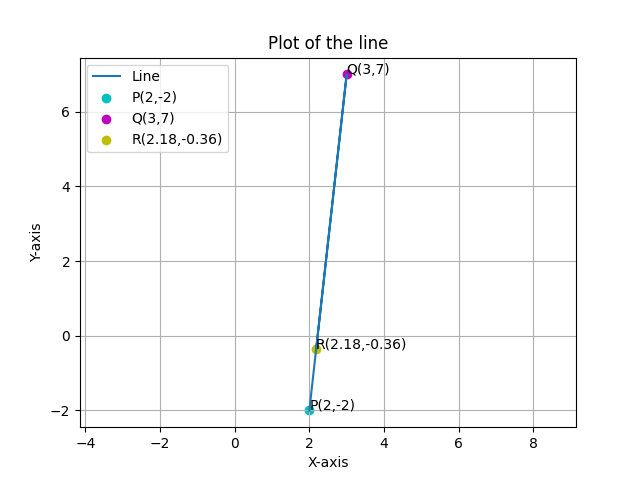
\includegraphics[width=0.7\linewidth]{figs/fig.png}
   \caption{Plot of the line}
   \label{stemplot}
\end{figure}


\end{document}

